\begin{frame}{Causal Analysis}
Example: Examining weight loss between new weight loss drug or placebo
 \begin{itemize}
  \item We would like to be able to say ``The drug leads to more weight loss''
  \begin{itemize}
   \item But need an RCT to say this
   \begin{itemize}
    \item Randomization minimizes differences between groups at baseline
   \end{itemize}

   \item We only have observational data
   \item Thus differences could be attributed to the drug or confounding
   
   \begin{itemize}
    \item e.g. healthier people were much more likely to take the drug at baseline
   \end{itemize}

  \end{itemize}
Idea: Try to balance the covariates to reduce the effects of confounding
so the two groups seem identical at baseline
 \end{itemize}
\end{frame}

\begin{frame}{Counterfactuals}
\begin{itemize}
 \item Suppose that for or every person, there are two potential outcomes
 \begin{itemize}
  \item $Y_i(0)$ - The outcome if they had taken the control, $T=0$
  \item $Y_i(1)$ - The outcome if they had taken the treatment, $T=1$
 \end{itemize}
 \item The observed value for subject i: $Y_i=Y_i(1)T+Y_0(1-T)$
  \end{itemize}
\end{frame}




  
\begin{frame}{Counterfactual Example}
   \begin{figure}[h!]
  \centering
    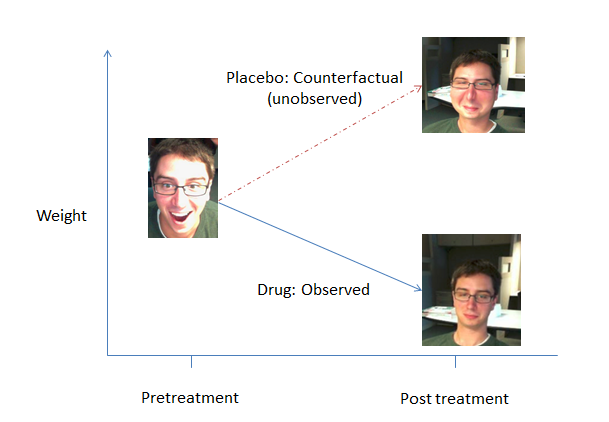
\includegraphics[width=0.5\textwidth]{counterfactual.png}
    \caption{Example of a counterfactual}
\label{fig:counterfactual}
\end{figure}

\begin{itemize}
 \item Obviously we only observe one. \textit{The fundamental problem of causal inference}
\item If we could observe both, then we could observe the causal effects for each person
\end{itemize}
\end{frame}

\begin{frame}{Rubin's Causal Model}
\begin{itemize}
\item Stable unit treatment value assumption (SUTVA): Treatment status of another subject does not affect outcome of other units. Single version of each treatment
\item Ignorability/No Unmeasured Confounders: $(Y(0),Y(1))\perp T|X$
\end{itemize}
\note{No association between outcome and treatment asignment}
\end{frame}




\begin{frame}{Estimands of Interest}
 \begin{itemize}
 \item Individual Treatment Effect: $Y_i(1)-Y_i(0)$
 \item Average Treatment Effect (ATE): $E[Y(1)-Y(0)]$. The effect of moving entire population
 from treated to untreated
 \item Average treatment effect for the treated (ATT): $E[Y(1)-Y(0)|T=1]$. The average treatment
 effect for those actually treated
 \item Note:  $E[Y(1)|T=1]\neq E[Y(1)]$, because $E[Y|T=1]=E[Y_1T+Y_0(1-T)|T=1]=E[Y_1|T=1]\neq E[Y(1)]$
\end{itemize}
 
\end{frame}


\begin{frame}{Propensity scores}
\begin{block}{Definition}
The propensity score is the probability that the subject received the treatment given the subjects \textit{pretreatment}
covariates. It is computed using the patient's baseline (pretreatment) information \cite{Rosenbaum1983}
\end{block}
 \begin{itemize}
  \item Defined as  $e_i(x)=P(T_i =1 |X_i)$
  \item Assume that the covariates play a role in how the subject chose treatment
  \item If we assume that $(Y(0),Y(1))\perp T|X \implies (Y(0),Y(1))\perp T|e(X)$, \cite{Rosenbaum1983}
  \item Controlling for propensity score will make groups seem indistinguishable
  \item Thus, we may treat it as if it were an RCT
 \end{itemize}

\end{frame}

\begin{frame}{Common Propensity Score Methods}
\begin{itemize}
 \item Matching: Match treatment and controls on their propensity score, calculate ATE
 \item Stratification: Stratify on propensity score, calculate ATE in each stratum
 \item Weighting: Weight each observation by the inverse of its propensity score, and then calculate ATE
 
  \begin{figure}[h!]
  \centering
    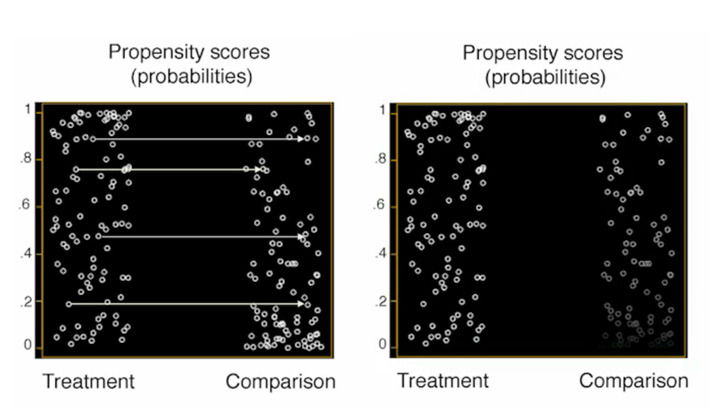
\includegraphics[width=0.8\textwidth]{ps_examples.png}
    \caption{Taken from TWANG shortcourse \cite{Rand2015}}
\label{fig:psexamp}

\end{figure}
\end{itemize}
\end{frame}

%ps issues was here
